%-------------------------------------------------------------------------------
% yum_configuration
%-------------------------------------------------------------------------------
%
% \file        yum_configuration.tex
% \library     Documents
% \author      Chris Ahlstrom
% \date        2016-03-07
% \update      2020-04-19
% \version     $Revision$
% \license     $XPC_GPL_LICENSE$
%
%     Provides descriptions of the configuration files.
%     Not yet part of the document.
%
%-------------------------------------------------------------------------------

\section{Configuration Files}
\label{sec:configuration}

   Let's cover the configuration files, which have expanded in utility in
   recent versions of \textsl{Yoshimi}.
   Understanding these configuration file makes it easier to
   use \textsl{Yoshimi}.
   Also note that all configuration settings are exposed to the command line
   interface as well.


   As with most applications, \textsl{Yoshimi} allows for one to save one's
   work and reload it. In recent versions of \textsl{Yoshimi}, it is possible
   to autoload a default state on startup, so that \textsl{Yoshimi} is
   already configured exactly as desired, with patches loaded and part
   destinations set.
   In addition, \textsl{Yoshimi} now saves settings that have been disabled.
   In this way, they can be re-enabled without having to reconstruct them from
   scratch.

   However, the configuration has changed quite a bit, and configurations from
   \textsl{Yoshimi} 1.4 and earlier will need to be reconstructed. With
   \textsl{Yoshimi} V 1.5.0 the following warning was devised, and will be updated
   with all major version number increments:

\begin{figure}[H]
   \centering
   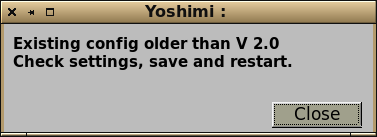
\includegraphics[scale=1.0]{2.3.0/configwarn.png}
   \caption{Configuration Warning Dialog}
   \label{fig:config_warn_dialog}
\end{figure}

   \textsl{Yoshimi} has a number of different files that make up the current
   configuration.
   Together, they make up the concept of a \textsl{patch set} (also called a
   \textsl{patchset}).
   Sometimes one will see reference to a "session", but that term is too easy
   to confuse with the "session" in "JACK session manager".
%  Here are the file extensions used for saving the \textsl{Yoshimi}
%  patch-set data:

   The last-used file in any configuration section is always at the top of its
   history list.  The main benefit of this new setup is that now all patch
   sets, vectors, scales, MIDI Learn, and state - offer the most recent entry
   when asked to load or save. On first-time use, when there is no history, one
   is offered one's home directory as a location, regardless of where
   \textsl{Yoshimi} was called from.  Presets are not yet included in this
   process.

   When saving these "managed" files, one won't be offered the previous
   last-used configuration unless it was seen during that session, either by
   being loaded, or saved by name.  This protects against accidental
   overwrites....

   For example, you've been working on 'foo' for a whole day, saving as you go,
   then the following day you start up \textsl{Yoshimi}, and immediately have
   a completely new idea 'bar', and start working on it. Without thinking you
   save and hit Enter. Oops, you just wiped out 'foo'. Only you haven't!
   At startup \textsl{Yoshimi} would not see the older file,
   so the save command just offers the home directory to put a new name in.

   Here is a summary of the files.  Please note that the names all start with
   \texttt{yoshimi}.  For example, \texttt{.banks} is really
   \texttt{yoshimi.banks}.

   \begin{itemize}
      \item \texttt{.banks}
         \index{.banks}
         \index{config!.banks}
         Contains information on the accessible instrument banks, and
         information to translate between bank directory names and bank ID
         values.
         Current root and current bank settings have now been moved from
         \texttt{banks} to the \texttt{config} and \texttt{instance}
         files, so the banks file now consists only of the bank structure.
         On first time start up, \textsl{Yoshimi} will look for
         \textsl{ZynAddSubFX} banks as well as \textsl{Yoshimi} banks in the
         usual locations. It \textsl{will not} look for a \textsl{ZynAddSubFX}
         configuration file, as these are no longer relevant.
      \item \texttt{.config}
         \index{.config}
         \index{config!.config}
         Contains the setup information configured in the
         \textbf{Yoshimi / Settings} dialog.
         This is just the basic configuration file.
         Configuration instances are now in place, so the main configuration
         file is common to all, but each instance has its own file for things
         like current bank, JACK/ALSA settings, etc.
         Common overall settings are only visible in the main instance and
         completely hidden in all the later ones.
         In \textsl{Yoshimi} V 1.6.1 there has been further revision of this.
      \item \texttt{.instance(n)}
         \index{.instance(n)}
         \index{config!.instance(n)}
         Contains the current root/bank, MIDI settings, and preferred engines.
         \textsl{Yoshimi} now has instance data separated from the main
         configuration file, with the name \texttt{yoshimi-(n).instance}.
      \item \texttt{.state}
         \index{.state}
         \index{config!.state}
         Contains the information needed to duplicate a complete \textsl{Yoshimi}
         session that was saved.
      \item \texttt{windows}
         \index{windows}
         \index{config!windows}
         Contains the current layout of windows for re-instation at the next
         startup of \textsl{Yoshimi}.
         If there is no such directory
         (\texttt{\textasciitilde/.config/yoshimi/windows}) then the
         keyboard is also opened, alongside the main window, as a help to those
         new to \textsl{Yoshimi}.
         And of course that state will be saved, if present, when
         \textsl{Yoshimi} exits.
         This directory is specific to the GUI, so doesn't really figure in
         this scheme, but it is created or saved when one exits
         \textsl{Yoshimi}.
   \end{itemize}
   The entire config set should then be (ignoring the prepended
   \texttt{yoshimi}):

   \begin{itemize}
      \item \texttt{.config}
      \item \texttt{.instance[n]}
      \item \texttt{windows}
      \item \texttt{.banks}
   \end{itemize}

   Before \textsl{Yoshimi} V 1.7.1 there was a single \texttt{.windows}
   file but now the directory called \texttt{windows} contains individual
   files with the status of each window recognised. This is more reliable and
   less prone to errors under fault conditions. Also, the main config
   directory is more rational.

   Other \textsl{Yoshimi} specific files are:

   \begin{itemize}
      \item \texttt{.xiz}
         \index{.xiz}
         \index{.xiz!Legacy format}
         \index{config!.xiz}
         An Instrument file.  This format is the \textbf{Legacy} or \textbf{Zyn}
         file format.  This format will be supported forever, although some
         backward-compatible refinements might be made as time goes on.
      \item \texttt{.xiy}
         \index{.xiy}
         \index{.xiy!Yoshimi format}
         \index{config!.xiy}
         An Instrument file in the new \textsl{Yoshimi} file format.
         This format includes all the
         controllers, the part mode status (Poly, Mono, Legato) and the
         Humanise settings.
         When loading files, \textsl{Yoshimi} will always look for
         the \texttt{.xiy} version first, and,
         if it can't find it, will then look for the \texttt{.xiz} version.
      \item \texttt{.xly}
         \index{.xly}
         \index{config!.xly}
         \index{MIDI Learn!.xly}
         A MIDI-Learn file for saving the MIDI-Learn settings in force at the
         moment this file is saved.  It is also included in the state file
         (\texttt{.state}).
      \item \texttt{.xmz}
         \index{.xmz}
         \index{config!.xmz}
         All \textsl{Yoshimi} active data; everything except MIDI-Learn.
         This file is called a \textsl{patch set}.
      \item \texttt{.xpz}
         \index{.xpz}
         \index{config!.xpz}
         Presets.
         A preset is a \textsl{Yoshimi} section of data stored by of the copy
         (C) controls. This may be an effect, part of an instrument etc.
      \item \texttt{.xsz}
         \index{.xsz}
         \index{config!.xsz}
         Scale Settings.
      \item \texttt{.xvy}
         \index{.xvy}
         \index{config!.xvz}
         Vector settings. The extension stands for "Xml Vector Yoshimi".
         Vector settings are now included in both the patch sets
         (\texttt{.xmz}) and state files (\texttt{.state}.
         For a good example, see \sectionref{subsection:vector_command_line}.
   \end{itemize}

   In the file-save dialogs, the file extension is determined by the type of
   file being saved, and it doesn't matter if one enters the extension
   explicitly, or not. If it's missing, or it is the wrong one, it will be
   replaced. This is actually true of almost all file saves, and has been for
   quite some time now.

   For vectors (in common with external instruments and patch sets),
   the configuration is saved to the user's home directory.
%  it's up to the user as to where to save.
%  The file filter generally defaults to the
%  either the user home directory, or if \textsl{Yoshimi} was launched from
%  userland, it's the directory it launched from. Then it's the normal
%  file browser selection.
   Once saved, \textbf{Vectors / Options / Recent} is your friend.

 %  \textsl{Yoshimi} can set up critical configuration settings to be writable
%   only by the main instance, but readable (and used) by any others. In the
%   current version of \textsl{Yoshimi}, this applies to \textbf{AddSynth
%   Oscillator Size}, \textbf{Internal Buffer Size}, and \textbf{Alsa
%   Samplerate}. These three must be defined before any other initialisation.

\subsection{Configuration Files / Patch Set}
\label{subsec:configuration_patch_set}

   \index{.xmz}
   \index{config!.xmz}
   \index{patch set}
   \index{file!patch set}
   A patch set is basically a group of instruments related simply by the user
   wanting to have them all loaded at once into \textsl{Yoshimi}.  A patch set
   is stored in a \texttt{.xmz} file.  A patch set is akin to a preset, in that
   it stores a combination of items, that took awhile to set up, for easy
   retrieval later.

   Patch sets are not the full configuration. They carry \textsl{most} of it,
   including almost all of the dynamic settings, but they don't contain the
   configuration settings that \texttt{.state} does.  The patch set format is
   either XML or compressed XML, as explained elsewhere.  The
   \textbf{Patch Sets / Save External...} menu entry saves files with
   the \texttt{.xmz} extension.

   One of the simplest ways to save one's work is to save the bulk of the
\textsl{Yoshimi} dynamic settings.
   This saving can be done through the \textbf{Patch Sets} menu,
   and will result in the creation of
   a \texttt{.xmz} file. Once created, this file will hold the settings for
   all settings within that setup, such as microtonal tunings, all
   patches, system effects, insertion effects, etc.
   See \sectionref{paragraph:menu_yoshimi_settings_main_settings}.
   Patch sets will save all other instruments regardless of whether they are
   activated or not.

   In many cases saving everything in a part is not what is desired.
   Saving a patch later on in an editing session is one such example.
   In order to save a patch, one can either save it from the
   \textbf{Instruments} menu, or through the \textbf{Bank} window.

\subsection{Configuration Files / Config}
\label{subsec:configuration_config}

   \index{.config}
   \index{config}
   \index{file!config}
   Often, one will see the extension \texttt{.config} used in the
   \texttt{\$HOME/.config/yoshimi} directory.  This file once contained
   information to translate between bank directory names and bank ID
   values.  In recent versions of \textsl{Yoshimi}, this file is much
   reduced in size, and its "doctype" is "Yoshimi".

   The \texttt{.config} file is always going to be specific to one machine and
   working modes, so no one will ever want to copy it across even to another
   \textsl{Yoshimi} environment.  Recent patch sets are now no longer stored in
   the main \texttt{.config} file, but in a new \texttt{recent} file.

%  see \sectionref{sec:local_data}.

   The \texttt{.config} file is now a much reduced common startup settings
   file.  It is a single file that every instance can read, but only the
   first one can write.

   The \texttt{.config} file has been separated from \texttt{.instance(n)}.
   It is saved only when the user explicitly calls for it to be saved. If
   it is missing for some reason when restarting, \textsl{Yoshimi} will
   report the fact and take corrective action.

   \begin{verbatim}
      $ yoshimi -a -A
      Yoshimi is starting
      ConfigFile /home/ahlstrom/.config/yoshimi/yoshimi.config not found, will
         use default settings ...
   \end{verbatim}

   The \texttt{.config} file will be readable by all instances of
   \textsl{Yoshimi}, but writable only by the main instance. The relevant
   controls will be hidden from the other instances.  Also, those controls not
   relevant to LV2 are disabled in that mode.  The \texttt{.config} and
   \texttt{.banks} data now reside in separate configuration files.  The banks
   file is saved every time there is a normal exit, so the last-used root and
   bank IDs will always match what that instance thinks is there.  Conversely,
   the main \texttt{.config} file \textsl{doesn't} get saved when one starts a
   new (unknown) instance of \textsl{Yoshimi}, but the config-changed flag is
   set, so one has control over whether any settings are saved.  So now, if
   anything goes wrong with the config files they won't corrupt one's carefully
   organised bank files, and vice-versa.

\subsection{Configuration Files / State}
\label{subsec:configuration_state}

   \index{.state}
   \index{config!.state}
   \index{state}
   \index{file!state}
   Sometimes one will see the extension \texttt{.state} used in the
   \texttt{\$HOME/.config/yoshimi} directory.  These files contain a lot
   more information that is needed to duplicate a \textsl{Yoshimi} session
   that was saved.  This file is a superset of an \texttt{.xmz} file,
   saving everything.
   The state file is accessed from the \textbf{State} menu item in the main
   window.
   Its default name is
   \texttt{\textasciitilde/.config/yoshimi/yoshimi.state}.
   This file can be auto-loaded when \textsl{Yoshimi} starts, if it is
   present and the feature enabled. Otherwise the normal settings are in
   place.

   The advantage of this is that one can set up a complete patch set of
   instruments one commonly uses, with all their settings, including audio
   destination.  Save it to the default state and it will be loaded, along
   with the system settings, every time one starts \textsl{Yoshimi}, if the
   \textbf{Yoshimi / Settings / Switches / Start With Default State}
   setting is checked. To revert the state, simply uncheck the
   \textbf{Yoshimi / Settings / Switches / Start With Default State}
   setting (and change any other needed).

   Since \textsl{Yoshimi} V 1.6.1 one specifically must \textbf{not} save
   the settings when changing this. It is part of the reorganisation.
   State, defaults, and jack session files have all been considerably
   improved, and behave in a more transparent fashion. Also, the instances
   have more controls available that can be actively restored.

   The \textsl{Yoshimi} 'state' file consists of the entire setup, (apart
   from basic configuration settings), instance to currently-loaded
   instrument sets. However, upon investigating some session managers, it
   looks like they don't want (or can't use) some of the configuration
   information because they are expecting to be able to change the entire
   state in \textsl{running} instances.

   \textsl{Yoshimi} now splits the 'instance' data
   from the main configuration.  This solves this session issue
   by saving only the true configuration locally, and to the state save.
   However, the 'instance' data includes things like ALSA/JACK settings.
   Since \textsl{Yoshimi} V1.6.1 one can change these
   \textsl{at the time the instance starts}, but there is a potential
   'gotcha'. If using the JACK session manager (and possibly others) it is
   possible to save a session to switch to ALSA audio when run, and this
   will be done. However, at that point the session manager loses contact
   with \textsl{Yoshimi} and it is no longer possible to save anything
   back to that session for that instance (assuming the session manager can
   handle multiple instances).

\subsection{Configuration Files / Instrument}
\label{subsec:configuration_instrument}

   \index{.xiz}
   \index{config!.xiz}
   \index{instrument}
   \index{file!instrument}
   An Instrument.  These files can have two formats, compressed and
   uncompressed.
   Uncompressed is set by
   \textbf{Yoshimi / Settings / Main Settings / XML Compression Level} set to
   0, and compressed is set by a value greater than 0.

   With the \textbf{Instrument} menu, one can save the file to any
   given location with the \texttt{.xiz} and/or \texttt{.xiy} extension.

   Default instruments are never saved, not even in patch sets and states, but
   if the parts are activated, that fact \textsl{is} saved; it's a part
   feature, not an instrument feature.

\subsection{Configuration Files / Scale}
\label{subsec:configuration_scale}

   \index{.xsz}
   \index{config!.xsz}
   \index{scale}
   \index{file!scale}
   Scale Settings.  These files store microtonal settings that \textsl{Yoshimi}
   can use to produce non-standard musical scales.  Recent scales settings are
   saved and recorded.


% \subsection{Configuration Files / Patch Sets}
% \label{subsec:configuration_patch_sets}

\subsection{Configuration Files / Instance}
\label{subsec:configuration_instance}

   \index{.instance(n)}
   \index{config!.instance(n)}
   \index{instance}
   \index{file!instance}
   A new feature of the \textsl{Yoshimi} configuration.
   It contains the current root/bank, MIDI settings, and preferred engines.
   These instance files are totally independent files, distinguished by a number
   in the file-name.

\subsection{Configuration Files / Banks}
\label{subsec:configuration_banks}

   \index{.banks}
   \index{config!.banks}
   \index{banks}
   \index{file!banks}
   A new feature of the \textsl{Yoshimi} configuration.  Currently each
   \textsl{Yoshimi} instance takes its own copy of the actual files as it starts
   up.  Previously, they could all save, delete, or rename the actual files without
   talking to the other instances, so one could move a file in one instance, and
   then try (and fail) to access it from another.

   For V 1.5.10 this issue was partially resolved by only allowing the main instance
   to make actual file changes (the related icons no longer existing in the
   other instances). However from V 1.7.2 this has been reverted as it was causing
   confusion, especially when \textsl{Yoshimi} was used as a plugin. The issue of
   all instances not being informed of a change made by the one currently in use
   will eventually be resolved.

   With the \textbf{Banks} menu, one can assign a patch to a given slot with
   a bank.  This instrument will remain in that slot for future use until it is
   deleted. To see the physical location of the \texttt{.xiz} file, one
   should check the
   \textbf{Yoshimi / Settings / Banks / Root Dirs}
   (\textsl{File / Settings / Bank\_Root\_Dirs}) window to see the paths for
   banks.

   At startup, after all the configuration is complete, the banks are loaded and
   installed.  On a per instance basis, the first thing this process does is
   look for a \texttt{yoshimi(-n).banks} file, if it can't, find that it then
   hunts for a \texttt{yoshimi(-n).config} file, and if that fails it does a
   re-scan for banks. In this way it should be completely backward compatible
   with any previous config files.

   The \texttt{.banks} file is \textsl{saved} every time roots, banks, or
   instruments are changed, and again on a normal exit to catch the current
   root and bank (which don't otherwise trigger a save).  This allows the
   last-used root and bank IDs to always match what that instance thinks is
   there.  Note that one needs to have write permissions to add instruments to
   the bank.  When one saves an instrument to a bank slot, it is given a
   filename with the internal name as the leaf-name.  When one saves an
   instrument to an external file, one is  first offered the internal name
   and the current directory, but one can change it if desired.

   By default, \textsl{Yoshimi} does not assign a bank ID 0 (zero) in any root.
   This feature has an interesting benefit. Several sequencers insist on
   setting a bank with every program change, and if one doesn't give a bank,
   they will try to set 0. However, \textsl{Yoshimi} is smart enough to ignore
   any invalid bank ID and remain with the existing bank number.

   As a further protection against rogue sequencers making assumptions, any
   attempt to set an invalid bank root will also be ignored.  On a
   first-time startup, discovered roots will be given ID numbers starting from 5,
   continuing in steps of 5. This makes it easier to re-arrange them to
   preference. We recommend not using 0.

   On first-time start up, \textsl{Yoshimi}
   looks for \textsl{ZynAddSubFX} banks as well, in the usual locations.
   It will not look for a \textsl{ZynAddSubFX} configuration file, as these
   are no longer relevant to \textsl{Yoshimi}.

   Banks are more thoroughly described in
   \sectionref{subsec:concepts_banks_and_roots}.

\subsection{Configuration Files / .bankdir}
\label{subsec:configuration_bankdir}

   A bit of ancient history has bubbled to the surface.
   When one creates a new bank in \textsl{Yoshimi}, it inserts an empty file in
   \index{config!.bankdir}
   the new bank, called \texttt{.bankdir}.  For example:

   \begin{verbatim}
      ... /banks/Zen Collection/.bankdir
   \end{verbatim}

   The reason for this is that when scanning for banks (especially at startup) it
   looks for this file first. If it can't find it, then it has to go though the
   slower process of looking for at least one completely valid instrument file.
   Running from SSDs, it probably won't make a lot of speed difference but it
   will on a conventional hard drive, especially if one has lots of banks.  So,
   if one wants to get that little startup edge, plonk a copy of this file into
      all your banks.  It's an empty file.

   In modern times, one of the main distros creates a warning for the packagers
   if it sees embedded dot files, and gets very unhappy if these are empty ones.
   The obvious answer is to put something there; \textsl{Yoshimi} now adds a
   \texttt{.bankdir} file that is useful -- when one creates a new bank, this
   file contains a string with the \textsl{Yoshimi} version number it was
   created with, and to add icing to the cake, every time one saves an
   instrument file in a bank, this file is updated and will have the current
   \textsl{Yoshimi} version number. Also, it will be created if it wasn't
   already there.

   So now it is be possible to tell how recently a bank was changed, which may
   have implications if running modern instruments on older \textsl{Yoshimi}'s.
   Also, the complaining distro will be happier because
   the \texttt{.bankdir} file won't be empty.

   For the "Collection" bank, the version number is now 2.0; although its
   instruments were created with \textsl{Yoshimi} sometime before version 1.3.0,
   some of the instrument files contain more information. "Drums" is set to 2.2.1;
   "Companion" is currently set to 2.2.0.

\subsection{Configuration Files / Windows}
\label{subsec:configuration_windows}

   \index{.windows}
   \index{config!.windows}
   \index{windows}
   \index{file!windows}
   No, this term isn't a reference to "that other operating system";
   it is a new feature of the \textsl{Yoshimi} configuration.
   It saves the current layout of application
   windows for re-instation at the next startup
   of \textsl{Yoshimi}.

\subsection{Configuration Files / Format}
\label{subsec:configuration_file_format}

   The Unix \texttt{file} command indicates that the XML files are one of
   two types:

   \begin{itemize}
      \item \textsl{exported SGML document, ASCII text}.
         These files are unindented XML data with an encoding of UTF-8 and
         a DOCTYPE of "ZynAddSubFX-data".
      \item \textsl{gzip compressed data, from Unix}.
         These files can be renamed to end in ".gz", and then run through
         the \texttt{gunzip} program to yield the XML file (but without an
         \texttt{.xml} extension).
   \end{itemize}

   The format depends on the "XML compression level" option discussed in
   \sectionref{paragraph:menu_yoshimi_settings_main_settings}.

   \index{saving settings}
   Saving settings or not:
   If one changes settings, and closes without saving, that means the settings
   remain in place only for the current session. If one has changed anything,
   when one closes \textsl{Yoshimi}, one will be given a second chance to
   save them. If one responds 'No',  the next time \textsl{Yoshimi} starts,
   the old settings will be restored.  An 'undo' feature would get pretty
   crazy very quickly.

   In the \textbf{Settings} window, \textbf{Save Settings}
   refers to the entire window, not just individual tabs. The close buttons are
   actually outside the frame of the tabs.

   \textbf{Close without saving} doesn't mean revert to previous settings; it
   means to use the changes, but don't immediately store them to the
   filesystem.

   In general, the contents are structured a lot like the
   user-interface elements that are used to set them.

\subsection{Configuration Files / MIDI Learn}
\label{subsec:configuration_file_midi_learn}

   \index{.xly}
   \index{config!.xly}
   The MIDI-Learn data crosses the border between static configuration and
   dynamic settings. It is stored in files with an extension of
   \texttt{.xly} ("XML Learn Yoshimi").
   If compression is turned off
   (\textbf{Yoshimi / Settings / Main Settings / XML Compression Level} set to
   0), this file is an XML/SGML file with a MIDILEARN section in it.

   When saving states, if there are any configured MIDI learned lines,
   these lines will also be saved.
   When one reloads the state they will also be restored.
   However, if the state file \textsl{doesn't} have any MIDI learn data,
   it \textsl{will not} clear any settings that are already there.

   Therefore, be aware that if one now re-saves that state, it \textsl{will}
   include such MIDI learned data, and the next time it is loaded,
   it \textsl{will} overwrite any lines that are already there.

   Also note that, during a master reset, the MIDI learn data is the only thing
   that \textsl{is not} cleared (unless the CTRL key is held down at the same
   time).

   These features are designed to give the best protection to a setup
   that could have taken quite a long time to arrange exactly as desired.
   In our experiments, we have discovered that we seem to use pretty much the
   same controls and actions, and the list of our 'preferred' settings is
   slowly increasing.

\section{Local Data Files}
\label{sec:local_data}

   \index{new!Local Data}
   During the development of \textsl{Yoshimi} V 1.7.1/2, a number of files and
   directories have been moved from the configuration directory to the
   standards preferred hidden directory in one's \texttt{home} directory.
   However, one's existing files in the old locations will be copied across, so
   there should be no disruption. For \textsl{Yoshimi} this is
   \texttt{.local/share/yoshimi}

   Here is a summary of the files.

\begin{itemize}
    \item \texttt{presets}
        \index{presets}
        User defined presets (or snapshots) are stored as individual files in
        the \texttt{presets subdirectory}.
   \item \texttt{recent}
         \index{recent}
         Recent instruments, patch sets, etc. are stored in the \texttt{recent}
         file. The last-used file in any section is always at the top of its
         recent history list.
    \item \texttt{found}
        \index{found}
        Editable copies of all the banks found in the \texttt{\textbackslash usr}
        installed locations are stored here.
    \item \texttt{\textasciitilde/.yoshimi\_history}
         \index{\textasciitilde/.yoshimi\_history}
         Specific to command line use, this holds the command-line history.
\end{itemize}

\subsection{Local Data Files / Presets}
\label{subsec:local_data_preset}

   \index{.xpz}
   \index{preset}
   \index{file!preset}
   Have a favourite setting for an envelope, or a difficult-to-reproduce
   oscillator? Then presets are for you! Presets allow for one to save the
   settings for any of the components which support copy/paste operations.
   This is done with preset files (\texttt{.xpz}), which get stored in the
   folders indicated by \textsl{Paths / Preset Dirs...}.
   The key thing about using presets is that one must first
   specify a presets directory!  Otherwise, who knows where they go?
   A good choice for a preset directory is
   \texttt{\textasciitilde/.local/share/yoshimi/presets}.
   In addition, copy-and-paste of synth settings can be done across
   \textsl{Yoshimi} instances.

   In \textsl{Yoshimi}, a
   \textsl{preset} is any collection of settings that can be saved to the
   clipboard or to a file, for later loading elsewhere.

   A preset is a canned version of a \textsl{Yoshimi} sub-setting.  Presets can be
   copied and pasted using the blue \textbf{C} and \textbf{P} user-interface
   buttons associated with many of the \textsl{Yoshimi} dialog windows.  They
   make it easy to save portions of the current settings for later use.  For
   example, resonance settings can be saved.

   The naming convention for a preset file is
   \texttt{presetname.presettype.xpz}, where
   \textsl{presetname} is the name one types into the \textbf{Copy to Preset}
   name field, \textsl{presettype} is the name that appears in the
   \textbf{Type} field, and \textsl{xpz} is the file-extension for compressed
   XML preset files.

   Since \textsl{Yoshimi} V 1.6.0 Preset 'root' directories are arranged in a
   similar way as bank roots, so one can zero in on just those of interest,
   with a 'current' directory instead of the previous 'default' one.
   \textsl{Yoshimi} instances can, of course, have their own current root, but
   the list of directories is common to all.

\subsection{Local Data Files / Recent}
\label{subsec:local_data_recent}

   \index{recent}
   \index{local!recent}
   \index{file!recent}
   Recently seen instruments, patch sets, etc. are stored in the
   \texttt{recent} file. For example, if the \textbf{XML Compression} option
   is set to 0, and one exits \textsl{Yoshimi}, then the following file might
   contain the following items (ignoring the XML markup):

   \texttt{\textasciitilde/.local/share/yoshimi/recent}

   \begin{verbatim}
      /home/me/yoshimi-cookbook/sequencer64/b4uacuse/yoshimi-b4uacuse-gm.state
      /home/me/sequencer64/contrib/yoshimi/horse.state
   \end{verbatim}

   \texttt{recent} is a single history file that every instance can read and
   write.

   This is actually quite interesting as there can never be a conflict.  It is
   impossible to have two browser lists open at the same time, and the lists are
   always rebuilt from memory every time they are opened. Similarly, the entries
   are added to every time a new recognised file is loaded or saved and one
   can't physically do two at the same time -- even if one could it would simply
   mean that one very briefly waited for the other, which is not an issue as
   they are not in the realtime thread.

   The \texttt{recent} file is saved only upon a normal exit, as it is
   comparatively unimportant.

\subsection{Local Data Files / Found}
\label{subsec:local_data_found}
   \index{new!Found Banks}
   Banks supplied when \textsl{Yoshimi} is installed are placed in read-only
   locations. This is inconvenient when one wishes to add to, or re-arrange
   them. From V 1.7.1, the first time these banks are seen they are copied into
   the local directory which \textbf{is} writable. For further details see
   \sectionref{subsubsec:banks_and_roots_bank_directories}

\subsection{Local Data Files / CLI history}
\label{subsec:local_data_cli_history}
   \index{Command Line History}
   The CLI history is an outlier and not part of the \textsl{Yoshimi} file
   management. It is a hidden file in one's \texttt{home} directory, maintained
   by the standard \texttt{readline} program.
   It conveniently allows you to easily repeat previous commands, both in the
   current session, and when restarting later ones.


%-------------------------------------------------------------------------------
% vim: ts=3 sw=3 et ft=tex
%-------------------------------------------------------------------------------
